\documentclass[12pt, psamsfonts]{amsart}

%-------Packages---------
\usepackage{amssymb,amsfonts}
\usepackage{fullpage}
\usepackage{tikz-cd}
\usepackage{todonotes}
\usepackage{physics}
\usepackage[all,arc]{xy}
\usepackage{enumerate}
\usepackage{enumitem}
\usepackage{mathrsfs}
\usepackage{theoremref}
\usepackage{graphicx}
\usepackage[bookmarks]{hyperref}

%--------Theorem Environments--------
%theoremstyle{plain} --- default
\newtheorem{thm}{Theorem}[section]
\newtheorem{cor}[thm]{Corollary}
\newtheorem{prop}[thm]{Proposition}
\newtheorem{lem}[thm]{Lemma}
\newtheorem{conj}[thm]{Conjecture}
\newtheorem{quest}[thm]{Question}

\theoremstyle{definition}
\newtheorem{defn}[thm]{Definition}
\newtheorem{defns}[thm]{Definitions}
\newtheorem{con}[thm]{Construction}
\newtheorem{exmp}[thm]{Example}
\newtheorem{exmps}[thm]{Examples}
\newtheorem{notn}[thm]{Notation}
\newtheorem{notns}[thm]{Notations}
\newtheorem{addm}[thm]{Addendum}
\newtheorem*{exer}{Exercise}

\theoremstyle{remark}
\newtheorem{rem}[thm]{Remark}
\newtheorem{rems}[thm]{Remarks}
\newtheorem{warn}[thm]{Warning}
\newtheorem{sch}[thm]{Scholium}

\DeclareMathOperator{\Hom}{Hom}
\DeclareMathOperator{\Id}{Id}
\DeclareMathOperator{\End}{End}
\DeclareMathOperator{\ord}{ord}
\DeclareMathOperator{\Aut}{Aut}

\makeatletter
\let\c@equation\c@thm
\makeatother
\numberwithin{equation}{section}

\bibliographystyle{plain}

\begin{document}

\title{Math 611 (Due 11/6)}
\author{Hidenori Shinohara}
\maketitle

\section{Simplicial and Singular Homology}

\begin{exer}{(Problem 14)}
  Determine whether there exists a short exact sequence $0 \rightarrow \mathbb{Z}_4 \rightarrow \mathbb{Z}_8 \oplus \mathbb{Z}_2 \rightarrow \mathbb{Z}_4 \rightarrow 0$.
  More generally, determine which abelian groups $A$ fit into a short exact sequence $0 \rightarrow \mathbb{Z}_{p^m} \rightarrow A \rightarrow \mathbb{Z}_{p^n} \rightarrow 0$ with $p$ prime.
  What about the case of short exact sequences $0 \rightarrow A \rightarrow \mathbb{Z}_n \rightarrow 0$?
\end{exer}

\begin{proof}
  Let $\phi_1: \mathbb{Z}_4 \rightarrow \mathbb{Z}_8 \oplus \mathbb{Z}_2, \phi_2: \mathbb{Z}_8 \oplus \mathbb{Z}_2 \rightarrow \mathbb{Z}_4$ be defined such that $\phi_1(a) = (2a, a)$ and $\phi_2(a, b) = a + 2b$.
  Then $\ker(\phi_1) = 0, \Im(\phi_1) = \ker(\phi_2) = \{ (2k, k) \mid 0 \leq k \leq 3 \}$ and $\Im(\phi_2) = \mathbb{Z}_4$.
  Thus this is indeed an exact sequence.

  \todo[inline,caption={}]{
    Finish this!
  }
\end{proof}

\begin{exer}{(Problem 15)}
  For an exact sequence $A \rightarrow B \rightarrow C \rightarrow D \rightarrow E$ show that $C = 0$ if and only if the map $A \rightarrow B$ is surjective and $D \rightarrow E$ is injective.
  Hence, for a pair of spaces $(X, A)$, the inclusion $A \rightarrow X$ induces isomorphisms on all homology groups if and only if $H_n(X, A) = 0$ for all $n$.
\end{exer}

\begin{proof}
  Suppose $C = 0$.
  $\Im(\phi_{AB}) = \ker(\phi_{BC}) = B$, so $\phi_{AB}$ is surjective.
  $\ker(\phi_{DE}) = \Im(\phi_{CD}) = \{ 0 \}$, so $\phi_{DE}$ is injective.

  On the other hand, suppose $\phi_{AB}$ is surjective and $\phi_{DE}$ is injective.
  $\Im(\phi_{CD}) = \ker(\phi_{DE}) = \{ 0 \}$, so $\phi_{CD}$ is the zero map.
  Therefore, $\ker(\phi_{CD}) = C$.
  $\ker(\phi_{BC}) = \Im(\phi_{AB}) = B$, so $\phi_{BC}$ is the zero map.
  Therefore, $\Im(\phi_{BC}) = 0$.
  Hence, $C = \ker(\phi_{CD}) = \Im(\phi_{BC}) = 0$.

  By Theorem 2.16 and the discussion at the bottom of P.117(Hatcher), we have a long exact sequence of homology groups
  \begin{align} \label{problem15_seq}
    H_n(A) \xrightarrow{i_*} H_n(X) \rightarrow H_n(X, A) \rightarrow H_{n - 1}(A) \xrightarrow{i_*} H_{n - 1}(X)
  \end{align}
  for $n \geq 1$.
  Suppose the inclusion induces isomorphisms on all homology groups.
  Then $H_n(X, A) = 0$ for all $n \geq 1$ by the first part.
  Moreover, we have $H_1(X, A) \rightarrow H_0(A) \rightarrow H_0(X) \rightarrow H_0(X, A) \rightarrow 0$.
  Since $H_1(X, A) = 0$, by the first part, $H_0(X) = 0$.
  In order for $0 \rightarrow H_0(X, A) \rightarrow 0$ to be exact, $H_0(X, A)$ must be 0.
  Therefore, $H_n(X, A) = 0$ for all $n \geq 0$.

  Suppose that $H_n(X, A) = 0$ for all $n \geq 0$.
  By exact sequence \ref{problem15_seq} above, $i_*: H_n(A) \rightarrow H_n(X)$ is surjective for $n \geq 1$ and injective for $n \geq 0$.
  Thus $i_*$ is bijective for all $n \geq 1$.
  We have $H_1(X, A) \rightarrow H_0(A) \rightarrow H_0(X) \rightarrow H_0(X, A)$.
  Since $H_1(X, A) = H_0(X, A) = 0$, $i_*$ must be bijective by the exactness.
  Therefore, the inclusion induces isomorphisms for all $n$.
\end{proof}

\begin{exer}{(Problem 16)}
  \begin{itemize}
    \item
      Show that $H_0(X, A) = 0$ if and only if $A$ meets each path-component of $X$.
    \item
      Show that $H_1(X, A) = 0$ if and only if $H_1(A) \rightarrow H_1(X)$ is surjective and each path-component of $X$ contains at most one path-component of $A$.
  \end{itemize}
\end{exer}

\begin{proof}
  $ $
  \begin{itemize}
    \item
      Let $\gamma_x + C_0(A) \in C_0(X) / C_0(A)$.
      Since $A$ meets each path-component of $X$, there exists a path $\gamma: I \rightarrow X$ that joins a point $a \in A$ and the image of $\gamma_x$.
      Then $\gamma$ can be seen as an element of $C_1(X)$ since $\gamma$ maps a 1-simplex into $X$.
      Moreover, $\partial\gamma = \gamma_x - \gamma_a$ where $\gamma_a \in C_0(A)$ with $\Im(\gamma_a) = a$.
      Therefore, $\partial(\gamma + C_1(A)) = \gamma_x + C_0(A)$, so $\gamma_x + C_0(A) \in \Im(\partial)$.
      Hence, $H_0(X, A) = \ker(\partial_0)/\Im(\partial_1) = (C_0(X)/C_0(A)) / (C_0(X)/C_1(A)) = 0$.

      On other hand, suppose that $A$ does not meet each path component of $X$.
      Let $x \in X$ be a point in a path component that $A$ does not intersect.
      Let $\gamma_x: \Delta^0 \rightarrow X$ such that $\Im(\gamma_x) = \{ x \}$.
      Then $\gamma_x \in \ker(\partial_0) = C_0(X, A)$.
      Let $\gamma + C_1(A) \in C_1(X, A)$.
      Then $\partial_1(\gamma + C_1(A)) = \partial_1(\gamma) + C_0(A)$.
      Let $\gamma_{x_1}, \gamma_{x_2} \in C_0(X)$ such that $\partial_1(\gamma) = \gamma_{x_1} - \gamma_{x_2}$.
      $\gamma_{x_1} - \gamma_{x_2} + C_0(A) \ne \gamma_x + C_0(A)$ if and only if $\gamma_{x_1} - \gamma_{x_2} - \gamma_x \in C_0(A)$.

      \begin{itemize}
        \item
          If $\gamma$ lies in the same path component as $x$, then so do $x_1$ and $x_2$.
          Suppose $x = x_1$.
          Since $-\gamma_{x_2} \notin C_0(A)$, $\gamma_{x_1} - \gamma_{x_2} + C_0(A) \ne \gamma_x + C_0(A)$.
          The case when $x \ne x_1$ and $x = x_2$ and the case when $x \ne x_1$ and $x \ne x_2$ can be proven in a similar way.
        \item
          If $\gamma$ lies in a different path component, then $\gamma_x \ne \gamma_{x_1}$ and $\gamma_x \ne \gamma_{x_2}$.
          Therefore, $\gamma_{x_1} - \gamma_{x_2} + C_0(A) \ne \gamma_x + C_0(A)$.
      \end{itemize}
      Therefore, $\gamma_x \notin \Im(\partial_1)$.
      Thus $H_0(X, A) = C_0(X, A) / \Im(\partial_1)$ is not 0.
    \item
      \todo[inline,caption={}]{
        Do part (b).
      }
  \end{itemize}
\end{proof}

\begin{exer}{(Problem 17)}
  $ $
  \begin{itemize}
    \item
      Compute the homology groups $H_n(X, A)$ when $X$ is $S^2$ or $S^1 \times S^1$ and $A$ is a finite set of points in $X$.
    \item
      Compute the groups $H_n(X, A)$ and $H_n(X, B)$ for $X$ a closed orientable surface of genus two with $A$ and $B$ the circles shown.
  \end{itemize}
\end{exer}

\begin{proof}
  $ $
  \begin{itemize}
    \item
      We will apply Theorem 2.16 to get the exact sequence with $H_n(A), H_n(X), H_n(X, A)$.
      \begin{itemize}
        \item
          When $n \geq 3$, $H_n(S^2) \rightarrow H_n(S^2, A) \rightarrow H_{n - 1}(A)$ shows that $H_n(S^2, A)$ is 0 by the exactness since $H_n(S^2) = H_{n - 1}(A) = 0$.
        \item
          When $n = 2$, $H_n(A) \rightarrow H_n(S^2) \xrightarrow{\phi} H_n(S^2, A) \rightarrow H_{n - 1}(A)$ shows that $H_n(S^2, A) = H_n(S^2) = \mathbb{Z}$.
          This is because $H_n(A) = H_{n - 1}(A) = 0$ so $\phi$ is an isomorphism by the exactness.
        \item
          \todo[inline,caption={}]{
            $n = 0$ and $n = 1$.
          }
      \end{itemize}

      \begin{figure}
        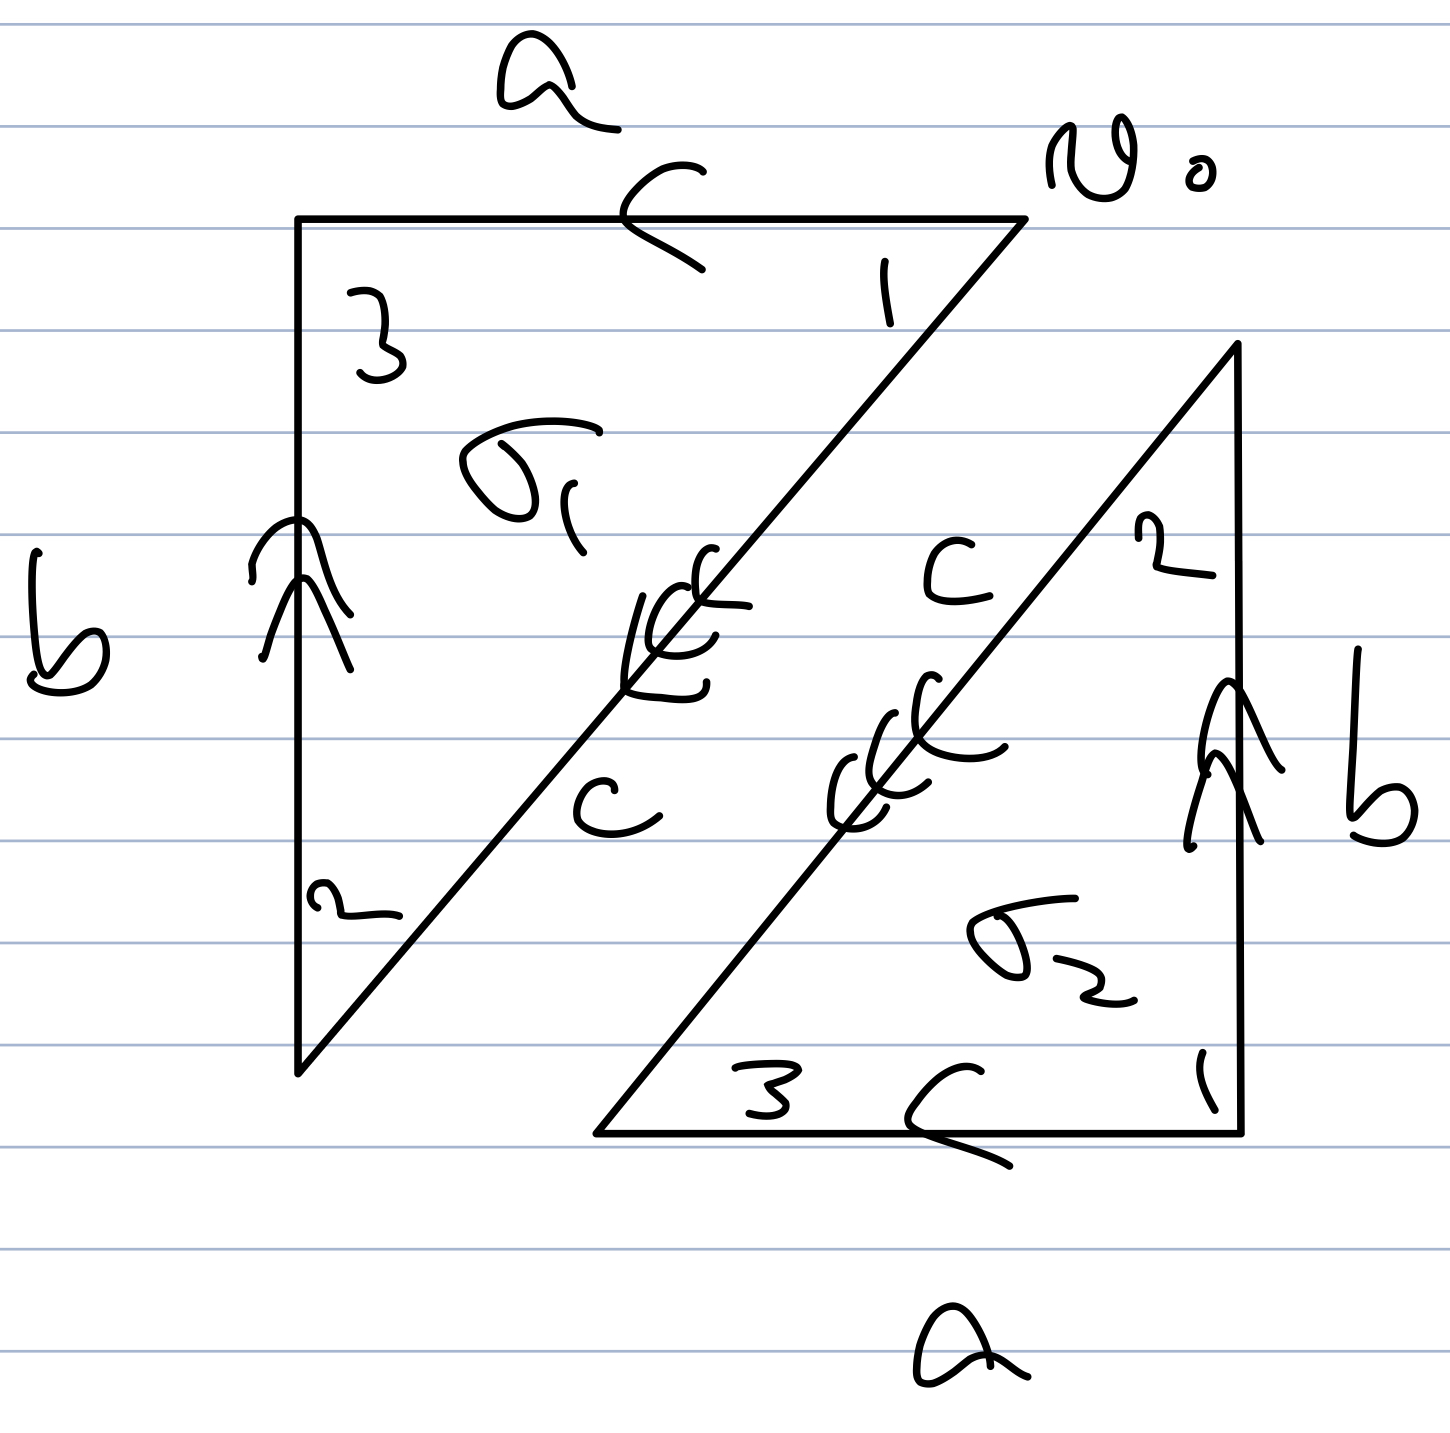
\includegraphics[width=.5\linewidth]{torus_homology.jpeg}
        \caption{Problem 17}
        \label{fig:torus_homology}
      \end{figure}
      We will first compute the homology groups of a torus using Figure \ref{fig:torus_homology}.
      $C_2 = \{ \sigma_1, \sigma_2 \}, C_1 = \{ a, b, c \}, C_0 = \{ v_0 \}$.
      \begin{itemize}
        \item
          $H_2 = \ker(\partial_2) / \Im(\partial_3) = \ev{ \sigma_1 - \sigma_2 } / 0 = \mathbb{Z}$.
        \item
          $H_1 = \ker(\partial_1) / \Im(\partial_2) = \ev{ a, b, c } / \ev{ b - a + c, c - a + b } = \mathbb{Z}^2$ because $b - a + c = c - a + b$.
        \item
          $H_0 = \ker(\partial_0) / \Im(\partial_1) = \ev{ v_0 } / 0 = \mathbb{Z}$.
     \end{itemize}

      Again, we will apply Theorem 2.16 to get the exact sequence with $H_n(A), H_n(X)$, and $H_n(X, A)$.
      \begin{itemize}
        \item
          When $n \geq 3$, $H_n(S^1 \times S^1) \rightarrow H_n(S^1 \times S^1, A) \rightarrow H_{n - 1}(A)$ shows that $H_n(S^1 \times S^1, A)$ is 0 by the exactness since $H_n(S^1 \times S^1) = H_{n - 1}(A) = 0$.
        \item
          When $n = 2$, $H_n(A) \rightarrow H_n(S^1 \times S^1) \xrightarrow{\phi} H_n(S^1 \times S^1, A) \rightarrow H_{n - 1}(A)$ shows that $H_n(S^1 \times S^1, A) = H_n(S^1 \times S^1) = \mathbb{Z}$.
          This is because $H_n(A) = H_{n - 1}(A) = 0$ so $\phi$ is an isomorphism by the exactness.
        \item
          \todo[inline,caption={}]{
            $n = 0$ and $n = 1$.
          }
      \end{itemize}

    \item
      \todo[inline,caption={}]{
        Finish this!
      }
  \end{itemize}
\end{proof}

\begin{exer}{(Problem 26)}
  Show that $H_1(X, A)$ is not isomorphic to $\tilde{H}_1(X / A)$ if $X = [0, 1]$ and $A$ is the sequence $1, 1/2, 1/3, \cdots$ together with its limit 0.
\end{exer}

\begin{proof}
  We will show that $H_1(X, A)$ is countable, and $\tilde{H}_1(X / A) = H_q(X / A)$ is uncountable.
  We have an exact sequence $\tilde{H}_1(X) \rightarrow \tilde{H}_1(X, A) \xrightarrow{\phi} \tilde{H}_0(A) \rightarrow \tilde{H}_0(X)$.
  Since $H_1(X, A) = \tilde{H}_1(X, A) = \tilde{H}_0(X) = 0$, $\phi$ is an isomorphism.
  Thus $\tilde{H}_1(X, A) = \tilde{H}_0(A) = \ker(\partial_1)/\Im(\partial_2)$.
  Since $A$ is a disjoint union of points, $\Im(\partial_2) = 0$.
  $\ker(\partial_1) = \{ \sum n_i\alpha_i \mid n_i \in \mathbb{Z}, \sum n_i = 0 \}$ where $\alpha_i$ is the point $1/i$ by the definition of a reduced homology.
  Then this is generated by $\{ \alpha_1 - \alpha_2, \alpha_1 - \alpha_3, \alpha_1 - \alpha_4, \cdots \}$, so $\tilde{H}_1(X, A)$ is countable.

  We will show the existence of an injective map $\zeta$ from the direct product $\prod_{i=1}^{\infty} \mathbb{Z}$ to $H_1(X / A)$, which is homeomorphic to the Hawaiian earring.
  We will refer to the $n$th ring $C_n$ as in Example 1.25.
  Let $(k_1, \cdots) \in \prod_{i=1}^{\infty} \mathbb{Z}$ be given.
  Construct the map $f: I \rightarrow X / A$ that wraps $k_n$ times around $C_n$ in the time interval $[1 - 1/n, 1 - 1/(n + 1)]$.
  This infinite composition of loops is certainly continuous at each time less than 1, and it is continuous at time 1 since every neighborhood of the basepoint in $X / A$ contains all but finitely many of the circles $C_n$.
  This shows that $f \in C_1(X / A)$.
  Moreover, $\partial(f) = v_0 - v_0 = 0$ where $v_0$ is the origin of the Hawaiian earring.
  Therefore, $[f] \in H_1(X / A)$.
  We define $\zeta(k_1, \cdtos) = [f]$.

  Let $(k_1, \cdots) \ne (l_1, \cdots) \in \prod_{i=1}^{\infty} \mathbb{Z}$ be given.
  Let $\zeta(k_1, \cdots) = f, \zeta(l_1, \cdots) = g$ as described above.
  Let $i$ be an index such that $k_i \ne l_i$.
  Let $F: X / A \rightarrow S^1$ be a continuous map that maps $C_n$ onto $S_1$ and $C_i$ to $-1$ for all $i$ where $S_1$ is seen as a subset of $\mathbb{C}$.
  Then $F$ induces a group homomorphism $F_* : H_1(X / A) \rightarrow H_1(S^1)$ where $F([f]) = k_n$ and $F([g]) = l_n$.
  Since $F([f]) \ne F([g])$, $[f] \ne [g]$.
  This shows the injectivity of $\zeta$ and hence $H_1(X / A)$ must be uncountable.

  Therefore, $H_1(X, A)$ is not isomorphic to $H_1(X / A)$.
\end{proof}

\end{document}


